\documentclass[tikz, border=10pt]{standalone}
\tikzset{
    vertex/.style = {
        circle,
        fill = black,
        outer sep = 2pt,
        inner sep = 1pt,
    }
}

\begin{document}

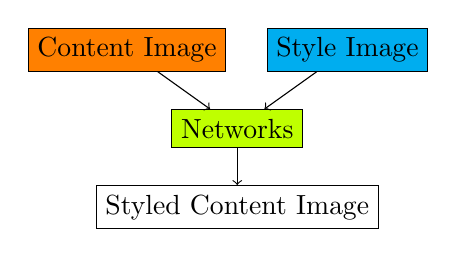
\begin{tikzpicture}

\node[draw,fill=orange](content image) at (0.6,0) {Content Image};
\node[draw,fill=cyan](style image) at (3.4,0) {Style Image};

\node[draw,fill=lime](networks) at (2,-1) {Networks};

\node[draw,fill=white](styled content image) at (2,-2) {Styled Content Image};

\draw[->,draw=black] (content image) to (networks);
\draw[->,draw=black] (style image) to (networks);

\draw[->,draw=black] (networks) to (styled content image);

\end{tikzpicture}

\end{document}